%----------------------------------------------------------------------------------------------------------
% Robotics safety report
%----------------------------------------------------------------------------------------------------------

\documentclass[10pt,a4paper]{article}
%----------------------------------------------------------------------------------------------------------
% Nödvändiga bibliotek
%----------------------------------------------------------------------------------------------------------

% Sånt man behöver för vanliga svenska dokument (byt tredje radens argument mot swedish istället för english för svenska dokument)
\usepackage[T1]{fontenc} %svenska tecken, åäö egna bokstäver
\usepackage[utf8]{inputenc} %vald teckenkodning
\usepackage[english]{babel} %engelsk dokumentstandard engelska rubriker

\usepackage[none]{hyphenat} %ta bort ordbrytning

\usepackage{hyperref} % göra länkar  

% För att bilder och tabeller ska hamna rätt
\usepackage{float}
\usepackage{algorithm2e}

% Mer för bilderna
\usepackage{graphicx}
%\usepackage{subcaption}
\usepackage{rotating}
\graphicspath{{images/}} %väg till bilderna

% Om man kanske vill räkna lite matte
\usepackage{amsmath}

% Figurpaket
\usepackage{tikz, tikz-3dplot}

\usetikzlibrary{arrows, decorations.markings}
\usetikzlibrary{shapes.geometric}

% För att texten inte ska hoppa in en bit i nya stycken
\setlength{\parindent}{0cm}
\setlength{\parskip}{0.25cm} %avtånd mellan stycken

%Skapa kommandot HRule som gör ett horisontellt streck 0.5 mm tjockt (används i titlepage)
\newcommand{\HRule}{\rule{\linewidth}{0.5mm}}

% Enables comment of blocks
\usepackage{comment}

%\usepackage{subfiles}

%----------------------------------------------------------------------------------------------------------
% Här börjar dokumentet
%----------------------------------------------------------------------------------------------------------

\begin{document}

\begin{titlepage}

\begin{center}   

% Title
{\Large CDIO Project - Images and Graphics }\\[1cm]

\HRule \\[0.4cm]% horisontellt streck
{\huge \bfseries Robotics Safety}\\[0.4cm]
\HRule \\[1.3cm]% horisontellt streck

%\includegraphics[width=\textwidth]{framsida}\\[1.4cm]

{\large Olle Fridolfsson\\
		Niklas Hansson\\
		Patrik Hillgren\\		
		Benjamin Ingberg \\
		Pär Lundgren\\
		Mattias Nilsson\\
		}

\vfill

% Bottom of the page
{\large \today}

\end{center}
\end{titlepage}

% Preamble

\section*{Preamble}

We would like to thank Johan Hedborg and Rickard Olsen for guidance and support throughout the project. A special thank to Eric Marcil at Yaskawa America Inc. for the help with configuring the controller. 
	% Förord, tack osv.
\pagebreak
\tableofcontents
\newpage

% Background - Despription of why this project is performed.
\section{Background}
This is the technical documentation of the work done by the Robotic Safety group in the course TSBB11 at Linköping University. TSBB11 is a CDIO project course given by the Computer Vision Laboratory where students apply their knowledge from previous theoretical courses in a larger project. The members of the group Robotic Safety all study the Signal- and Image Processing master program. 
The project assigned to the group is in the area of robotics safety and is requested by IEI (Department of Management and Engineering) at Linköping University and relates to the robot SIA20D Motoman by Yaskawa Nordic. 

% Closer description of poject

\section{Project Description}
Robots like the SIA20 Motoman are powerful and can in some situations cause harm to humans working in the same area. The goal of this project is to create a system which ensures a safe environment in a human robot collaboration area. This will be done by determining the distance between the closest moving object and the robot and retrieve a control signal to send to the robot depending on that information. The control signal should determine four states:
\begin{enumerate}
\item The closest moving object is outside safety zone 2 (see figure below). Objects are not in the collaborative area, the robot can work at standard motion. 

\item The closest moving object is within safety zone 2. This means that the robot motion shall be reduced since the moving object is within the collaborative area.

\item The closest moving object is within safety zone 1. This means that the robot must stop.

\item The closest moving object is within the emergency zone. This means that the robot must perform an emergency stop, which differs from the usual stop. 
\end{enumerate}

\begin{figure}[H]
\begin{center}
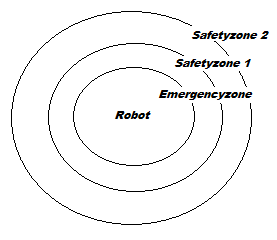
\includegraphics[width=7 cm]{robotsafetyzone}
\caption{Scheme of the different zones}
\label{robotsafetyzone}
\end{center}
\end{figure}


% Description on the libraries on environment used.

\section{Development Environment}

% Overview of how the programm is structured

\section{System Overwiev}

For monitoring the area surrounding the robot a Microsoft Kinect is used. Together with data that is received from the controller it is possible to decide whether a visible object is within a safe distance from the robot, or not. The data from each source is transformed into a joint environment.

The system consist of:
\begin{itemize}
\item A Kinect - a motion sensing input device by Microsoft.
\item Yaskawa DX100 controller - provided with a MotoPlus application.
\item Yaskawa SIA20 robot - A slim version of it predecessor IA20.
\item A Computer running the system.
\end{itemize}

\begin{figure}[H]
\begin{center}
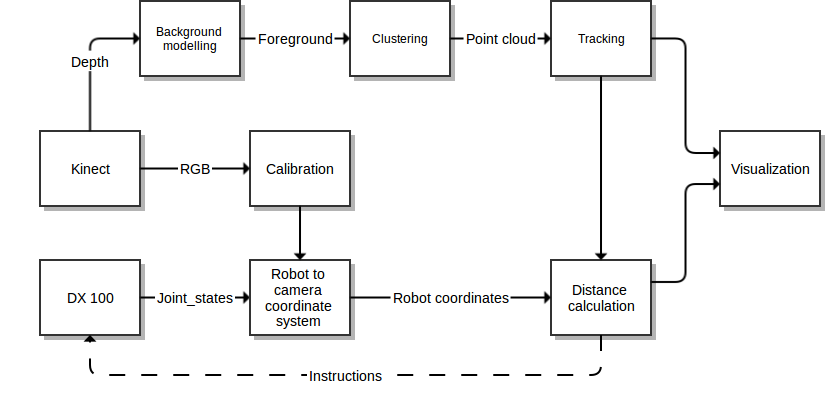
\includegraphics[width=15 cm]{flowchart}
\caption{Flowchart of system}
\label{flowchart}
\end{center}
\end{figure}




From the Kinect a depth image is provided. A background model algorithm is applied on the depth image and a foreground is obtained. The foreground only consist of moving pixels and is fairly rough. Therefore a clustering algorithm is used to extract only the relevant data. Clusters are easier to handle and much easier to track. Tracking provides a backup for what the background model might fail on. E.g. since objects might be left out from the foreground if they stay at the same place for too long.

The Kinect also provides an RGB image which makes it possible to perform calibration of the camera extrinsics using calibration patterns. Calibration algorithms are used to find transformations between different coordinates systems. This is crucial in order to measure the distance between the robot and an object.

The visualization displays a point cloud of the objects together with the robot model. Lines are used to represent the closest point pairs. The color of the line indicates in which zone the object is situated. Red emergency zone, yellow safety zone 1 and green safety zone 2.

The original idea was to send instructions to the controller. However integrating the robot in the system ended up being very time consuming. Since the topic of this project is computer vision and image processing the group decided to leave the instruction sending part out. It is possible to further develop the project to include robot control based on decisions made by our system.   




\section{Subsystems}
This section describes in detail the different parts which are included in the system.
% Input data 
\subsection{Input Data}
\subsubsection{Joint states of robot}
When connection with the controller is established the joint states will be available. Each joint has a value in radians describing its state, i.e. its revolution. The objective is to build a model of the robot in camera centered coordinates where the distance to a moving object, represented as a point cloud in 3D space can be computed.
The data regarding joint states is used for both visualization, in the shape of a mesh figure, and for calculation of the robot's position in relation to other objects. These two are independent with respect to each other.

\subsubsection{Depth-image from Kinect}
The IR projector and IR camera provides a depth image of the collaboration area. The data is used for background segmentation and calibration. 

\begin{figure}[H]
\begin{center}
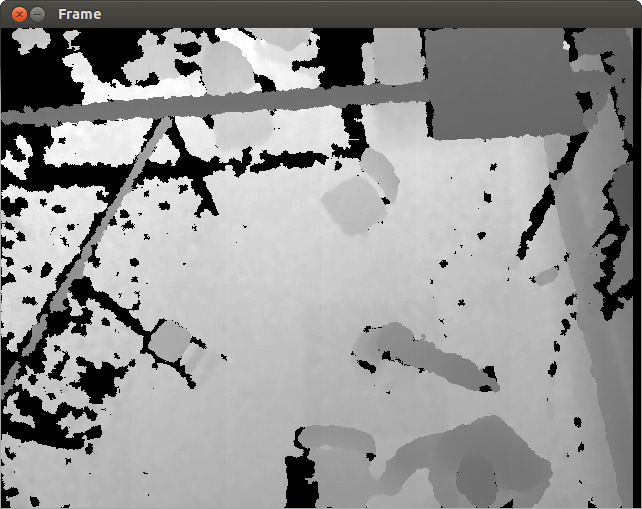
\includegraphics[width=12 cm]{screenshot_depth_image}
\caption{Depth image}

\end{center}
\end{figure}

\subsubsection{RGB-image from Kinect}
The RGB camera is used for calibration of both intrinsic and extrinsic camera parameters. From those it is possible to determine a relationship between the camera and a well known positioned calibration pattern. 

\begin{figure}[H]
\begin{center}
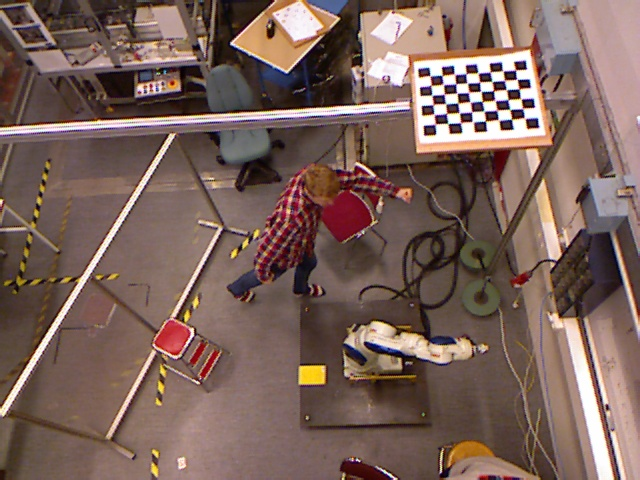
\includegraphics[width=12 cm]{image_color}
\caption{RGB-image}

\end{center}
\end{figure}


% Calibration between coordinate systems.

\subsection{Calibration}
To relate the camera system to the world system defined by a fixed point in a calibration pattern the system has to be calibrated. For calibration of the camera intrinsic parameters and distortions from the pinhole camera model the system uses the models and methodology described by Zhang, 2000 \cite{zhang}. This is performed offline.

For online calibration of the camera extrinsics the same distortion and intrinsic parameters are used with a world fixed calibration pattern.

The online calibration is very computationally expensive however since the system is supposed to be stationary, recalibration is only done once a second to compensate for small adjustments on the system. The possibility for the camera to move still exists and if so the system would be maladjusted and give out wrong answers which is why the online calibration is performed.

Most of the building blocks of the calibration is implemented by the OpenCV library \cite{camcal}. 

\subsubsection{Intrinsic calibration}
Before image distortions the projection of the 3D-world to the image plane is described by this matrix:

\[\begin{bmatrix}
x \\
y \\
w
\end{bmatrix}
=
\begin{bmatrix}
 f_x & 0   & c_x \\ 
 0   & f_y & c_y \\ 
 0   & 0   & 1
\end{bmatrix}
\begin{bmatrix}
X \\
Y \\
Z
\end{bmatrix}\] 

Where $f_x$ and $f_y$ are the number of pixels per unit of length, $c_x$ and $c_y$ are the center pixel coordinates of the image. X, Y and Z are the camera relative positions of a visible point with x, y and w as the homogeneous representation of the pixel coordinate where the point is projected.

Distortions from this model is modelled as radial distortion as well as tangential distortions. Radial distortions produce a fish-eye effect on the image and is compensated for with this model:

\[x_{radialcorrected} = x\cdot (1+k_1\cdot r^2 + k_2\cdot r^4 + k_3\cdot r^6)\]
\[y_{radialcorrected} = y\cdot (1+k_1\cdot r^2 + k_2\cdot r^4 + k_3\cdot r^6)\]

Tangential distortions due to the lense not being perfectly aligned is compensated with this model:

\[x_{tangentialcorrected} = x + 2p_1xy+p_2(r^2+2x^2)\]
\[y_{tangentialcorrected} = x + p_1(r^2+2y^2)+2p_1xy\]

Since this is a standard model external libraries have support for these parameters and the error correction from calculating the distortion parameters will cascade into other functions. Intrinsic and distortion calibration is done offline and the parameters are saved into a YAML file.

\subsubsection{Extrinsic calibration}
To relate the position and state of the robot to the camera there needs to be a reference between a fixed robot frame and the camera frame. To solve this a calibration pattern is placed at a known position relative to the robot.

This calibration pattern is then detected in the image and the solution to the PnP (Perspective-n-Point) problem with the camera parameters is used as extrinsic parameters.

To minimize noise and increase robustness a large chessboard pattern with 6x8 known points is used for calibration. However there is no known analytical solutions to the PnP problem for n > 3 so the problem is solved using optimization (minimization of the sum of squared reprojection errors) with the Levenberg-Marquardt iterative optimization algorithm.

To prevent the optimization getting stuck on local optima the system uses initial solutions provided by the P3P solver.
The points used for these initial solution are the four corners of the chessboard, three to solve the P3P problem and one to validate which of the four possible solutions is consistent with the rest of the data.
The P3P solver used in OpenCV provides an unknown number of solutions since the algorithm does not handle all possible cases. 

The PnP solver then uses these initial solutions to find the optimal solution.
To verify that the provided solution is correct the system checks that the x-axis in the found coordinate system is flipped compared to the x-axis specified by the camera.
This is necessary due to the problem of unknown numbers of solutions from the P3P solver.


\subsubsection{tf}
The tf subsystem is a built in part of ROS for managing transformations between different coordinate systems. It is written and maintained by Tully Foote. The tf package takes the different transformations of the system as input. Using them it can then provide the position of a point in an arbitrary coordinate system at any point in time.

\subsubsection{Transformation of robot joints}
Since information regarding the design of the robot is provided the transformations between the joints can be obtained. The tf package then makes it possible to transform the robot and its joints into a given coordinate system.

\subsubsection{Transformation into camera coordinate system}
A static transformation between calibration pattern and the base of the robot in world coordinates is set. Given the transformation from camera to calibration pattern, it is possible to transform each joint to the camera coordinate system. This results in a set of joints on which the distance calculation to moving objects in the scene can be performed. 



\subsection{Background segmentation}

The background segmentation node is based on the backgroundSubtractorMOG2 from OpenCV \cite{BGS} which uses Gaussian mixtures to perform the segmentation. The background segmentation results in a binary image of the foreground. The background modelling uses statistical properties by model each pixel as a mixture of gaussians. A pixel is counted as foreground when it deviates from these gaussians. Checking each pixel in the frame gives out the entire foreground. The background model updates for each frame processed which means it is computationally expensive. 

\begin{figure}[H]
\begin{center}
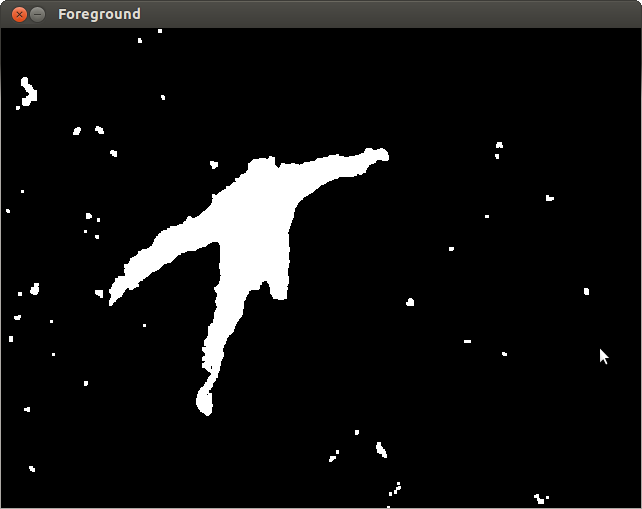
\includegraphics[width=12 cm]{screenshot_foreground_image}
\caption{Foreground from background segmentation}

\end{center}
\end{figure}


The foreground and depth image are used to construct a point cloud. For each foreground pixel the corresponding depth value $Z$, pixel coordinates $x$, $y$ and intrinsic parameter can be used to obtain the world coordinates as follows.

\begin{center}
$\displaystyle X = (x - c_x) \cdot \frac{Z}{f_x}$\\ \vspace{10 pt}
$\displaystyle Y = (y - c_y) \cdot \frac{Z}{f_y}$

and the 3D point is ${\bf P} = [X, Y, Z]^T$
\end{center}


By applying these formulas to all foreground pixels the point cloud is obtained.




%Clustering of point cloud

\subsection{Clustering}
Clustering
The clustering node receives a point cloud from the background segmentation node corresponding to the extracted foreground i.e. moving objects. The purpose of the clustering node is to divide the entire point cloud into individual objects. It also removes noise and objects that are not considered to be large enough.  

The reason why individual objects are necessary is because the closest distance to every object compared to the robot is desired. It is not sufficient to know the distance from the closest point in the whole point cloud to the robot. Separating the entire point cloud into individual clouds also provides the possibility for an implementation of tracking point cloud objects. 

The separation of objects is done by separating the entire point cloud into clusters. This is done using an euclidean cluster extraction algorithm. A simple outline of the algorithm is that for each point, check whether there is another point within a given radius and if so assign this point to the same cluster. In other words, the points that are close enough are concatenated to each other. If there is no point within the given radius that already is assigned to a cluster then the point should correspond to a new cluster. The cluster extraction is based on the algorithm given by Point Cloud Library \cite{CE}.

\subsection{Removal of Robot}

In the background segmentation the system finds everything that is classified as foreground, including the robot. This results in a point cloud that might contain values corresponding to the robot. The purpose of this project is to check if detected objects are within a certain distance from the robot. If the robot itself is one of the objects the distance will always be minimal and the system will not work. This means that the system needs to remove clusters corresponding to the robot from the other clusters before it can calculate distances and make a decision. 

Removing the clusters corresponding to the robot is done by using the joint coordinates of the robot. Since the system only knows the joints position and not the entire hull of the robot the first thing that needs to be done is to create a convex hull corresponding to an approximation of the real hull of the robot. The approximated hull is achieved by creating lines between connected joints and applying a cylinder around these lines. The radius of the cylinder is given by the greatest radius of the robot between these joints. In other words the cylinders corresponding to the hull of the robot will cover up the whole robot. After the hull is created a simple check is performed which finds out if a certain amount of the points in a cluster are inside any of these cylinders. If this is the case these clusters are excluded for further processing. It is not trivial to know if a point is inside a cylinder, the used method is copied from Greg James. \cite{cylinder} The pseudo code for the algorithm is described below.

point 1= the point that is checked if it is inside a cylinder
point 2= the first point of the cylinder 
point3=the second point of the cylinder
vector= the vector from point 2 to 3.
%1. Translate point1 so that point2 lies in the origin.
%2. Check if the dot product point1*vector is positive and smaller than |vector|^2
%3. If it is not, it is outside the cylinder horizontally.
%3. Calcu


\begin{figure}[H]
\tdplotsetmaincoords{60}{120}
\begin{tikzpicture}
	[scale=5,
		tdplot_main_coords,
		axis/.style={->,black,very thick},
		vector/.style={-stealth,black,very thick},
		vector guide/.style={dashed,black,thick}]

	%standard tikz coordinate definition using x, y, z coords
	\coordinate (O) at (0,0,0);
	%\coordinate (v) at (1,1,1.5);
	%\coordinate (c1) at (0.1,0.1,0);
	%\coordinate (c2) at (1.5,1.5,0.5);
	
	%tikz-3dplot coordinate definition using r, theta, phi coords
	\tdplotsetcoord{v}{1.5}{55}{55}
	\tdplotsetcoord{c2}{1.5}{90}{55}
	%draw axes
	\draw[axis] (0,0,0) -- (1,0,0) node[anchor=north east]{$x$};
	\draw[axis] (0,0,0) -- (0,1,0) node[anchor=north west]{$y$};
	\draw[axis] (0,0,0) -- (0,0,1) node[anchor=south]{$z$};
	
	%draw a vector from O to P
	\draw[vector] (O) -- (v);
	\draw[vector] (O) -- (c2);
	\draw[vector guide] (v) -- (vxy);
    \draw[vector] (O) -- (vxy);
	%\draw[vector guide] (c2) -- (vxy);
	
	%\draw (v) circle[radius=2pt];
	\fill (v) circle[radius=0.15mm];
	\fill (vxy) circle[radius=0.15mm];

	\fill (c2) circle[radius=0.15mm];
	
\node[above right] at (vxy) {\hspace{5 pt}$\mathbf{v_1 = v^Te\cdot e}$};
\node[right] at (v) {\hspace{10 pt}$\mathbf{v=p-c_1}$};
\node[right] at (c2) {\hspace{10 pt}$\mathbf{e=c_2-c_1}$};

\end{tikzpicture}
\caption{Geometry for computing the orthogonal distance to a vecor}
\label{geometry}
\end{figure}
\vspace{20 pt}


The objective is to conclude if {\bf p} is inside a cylinder with squared radius $r^2$ and endpoints ${\bf c_1}$, ${\bf c_2}$. First ${\bf c_1}$ is subtracted from all points to get the vectors shown in figure \ref{geometry}. $\bf v_1$ is obtained by projecting $\bf v$ onto $\bf e$ The condition that ${\bf v}$ is in between the caps (endpoints) of the cylinder is the following:\\
 $ 0 < {\bf v}^T{\bf e} < \| {\bf c_1}-{\bf c_2}\|$ if this is not fulfilled this distance is discarded. Otherwise the orthogonal squared distance using pythagoras formula is\\
$\displaystyle d^2 = \|{\bf v}\|^2 - \|{\bf v_1}\|^2= {\bf v}^T{\bf v} -\frac{({\bf v}^T{\bf e})^2}{{\bf e}^T {\bf e}}$ if $d^2 < r^2$ the point is inside the cylinder



\subsection{Distance Calculation}

% Tracking of Objects

\subsection{Tracking}
The system uses a background segmentation which has a learning rate. This means that the system  adapts its considered background during runtime. Since the system is adaptive, people who are standing still will disappear after a while. For that situation the system is not safe. This problem is solved by tracking objects found in the scene. 

%The tracking algorithm will save information of objects that disappears in the scene and the %robot will not continue working in normal pace until the object has left the safety zone. The %system is not required to keep track of objects that is occluded and objects that interfere %with each other. Since the requirement of the tracker is rather low the implementation is %simple and has no guarantees of actually tracking objects throughout the entire scene if %occlusion occurs.

To keep track of all objects in the scene an object list is used to contain information about all objects. The information describes for all objects the relationship to the robot, the mean point of the cluster and if it is visible or not. 

%and an index towards the object which is closest to the robot. Every object contains the %closest joint on the robot, closest point on the object and the distance between them, which 
%is called the min-distance. It will also contain an average point and a bool-variable which %tells if the object is visible or not.  

Every cluster which is classified as an object will then correspond to an object in the object list. When an object is calculated in a new frame its average point will be compared to the average points of the objects in the object list. If there are any objects in the object list which does not correspond to any objects in the current frame there are theoretically two different possibilities, the object has moved out of the camera view or the object has blended into the background. To know which one it is the min-distance of the object is used. If the distance is sufficiently large it is assumed that the object has moved out of the camera view and the object will then be removed from the object list. If the distance is sufficiently small the object is assumed to have blended into the background, the object will then be kept in the object list but it will be marked as not visible. Objects that are outside the safety zones will not be tracked. Since new objects can not occur inside the safety zones another advantage with the tracking is that it will reduce noise.

\begin{figure}[H]
\begin{center}
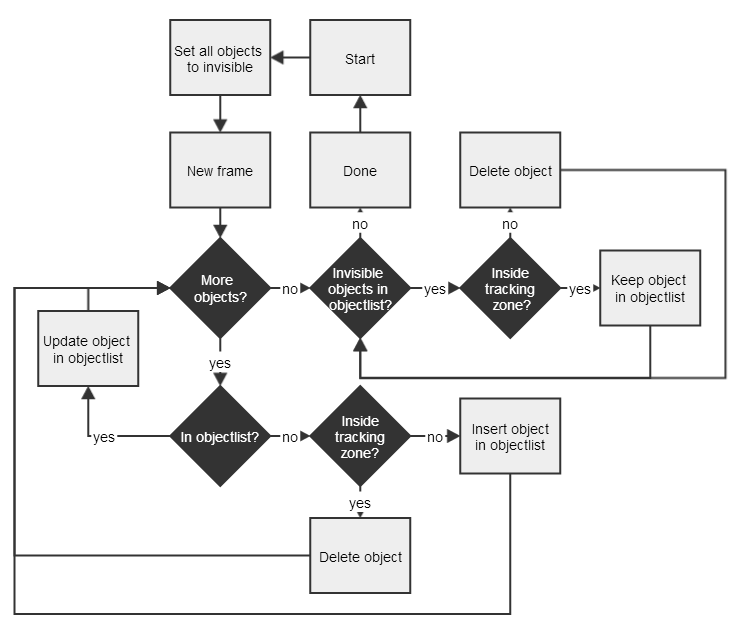
\includegraphics[width=12 cm]{tracking}
\caption{Flowchart of tracking algorithm}
\label{tracking}
\end{center}
\end{figure}


\subsection{Visualization}

The results of the system is visualized in RViz, which is a 3D visualization tool for ROS. 

\subsubsection{Robot}
The data received from the controller are the joint states.
The visualizer, RViz, uses these states when determining the robots pose.
The robots construction is predefined and RViz only requires the joint states to draw the robot.
The length between the nodes and its appearance was provided by developer, in mesh format.
 
\begin{figure}[H]
\begin{center}
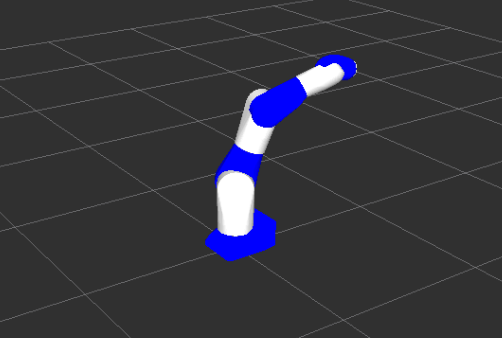
\includegraphics[width=12 cm]{robot}
\caption{3D-model of robot.}

\end{center}
\end{figure}

\subsubsection{Objects}
The objects in the image that the tracking algorithm considers being real moving objects are visualized. They are published as point clouds so that Rviz can subscribe to them and visualize them. If the tracking algorithm believes that an object has disappeared because of non-movement, it keeps the last seen point cloud of the object i.e. static objects in the scene are objects that the system thinks are standing still. 

\begin{figure}[H]
\begin{center}
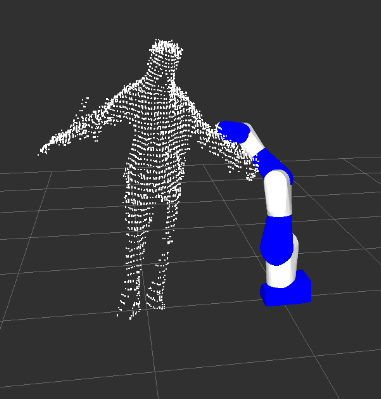
\includegraphics[width=12 cm]{humanandrobot}
\caption{Clustered object beside the robot.}

\end{center}
\end{figure}


\subsubsection{Distances}
To visualize the resulting state of the system (the current safety zone) a line between the closest object and the closest joint of the robot is drawn. This line switches color depending on which state the system is in. The color of the line is thereby the result of the system. 

\begin{itemize}
  \item Red - Emergency zone
  \item Yellow - Safety zone 1 
  \item Green - Safety zone 2
  \item No line - Outside safety zone 2 
\end{itemize}

\begin{figure}[H]
\begin{center}
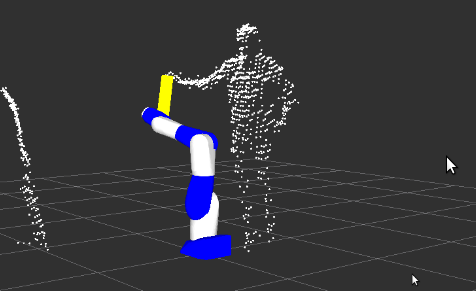
\includegraphics[width=12 cm]{resultat1}

\caption{Result}
\end{center}
\end{figure}

\begin{figure}[H]
\begin{center}
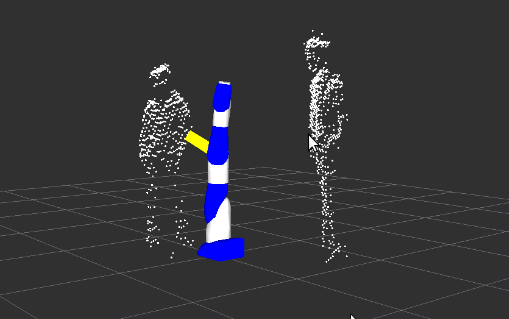
\includegraphics[width=12 cm]{resultat2}

\caption{Result}
\end{center}
\end{figure}


\section{Results and Evaluation}
In this type of project there is no typical solution which final results can be evaluated by comparing the results with ground truth values. This is simply because there is no ground truth available for this type of problem. Evaluation of the system must then be done by checking if the system works for all possible scenarios. This type of evaluation is not quite desirable since it will not give a result which can be compared to other implementations of the same or similar problem. However, it will give a good understanding if the system works or not and motivates if the system could be used in real life collaboration areas between robots and humans. The following scenarios have been evaluated:

1. A person walks in into the scene, enters the outer security zone, stops and then leaves. This is the most trivial test and will show if the system produces any valuable results. This situation should be tested from all directions and the test person should enter all zones. 

2.  A person walks in into the scene, enters the outer security zone, stops for a long period of time and then leaves. This situation should be tested from all directions and the test persons should enter all security zones.

3. Two persons enter the scenes, enters the outer security zone, stops for a short period of time and then leaves. This situation should be tested from all directions and the test persons should enter all security zones. The path of the two persons should not interfere with each other, that is keeping a clear distance from each other. 

4. Two persons enter the scenes, enters the outer security zone, stops for a short period of time and then leaves. This situation should be tested from all directions and the test persons should enter all security zones. The path of the two persons should interfere with each other, that is at one point keep a very small distance between each other. 

5. A person enters the scene, enters the outer security zone, stops for a short period of time and then leaves. Before the person leaves it leaves an object behind within the outer security zone. 

6. Two persons enter the scene maintaining physical contact (enough for them to appear as one object in the cluster extraction), enters the outer security zone, terminates the physical contact (the cluster extraction should now extract two objects) and then both leave the scene.

7. Two persons enter the scene maintaining physical contact (enough for them to appear as one object in the cluster extraction), enters the outer security zone, terminates the physical contact (the cluster extraction should now extract two objects) and then one person leaves the scene while the other stays in the outer security zone.


8. Multiple persons enters the scene acting like a herd of sheeps (moving randomly without knowledge about the robot). The persons should once in a while enter security zones. This test makes it possible to count the number of correct classifications and this test more or less correspond to a real life situation. 

\subsection{Performance of system using tracking functionality}
The tracking algorithm performs very well when a single object is within the collaborating area.
The tracker stays with the object and holds on to it, even when it is no longer visible in the foreground.\\

A person can enter the area, have its distance to the robot visualized with either a green, yellow or red marker.
The marker is illustrated in form of a cylinder between the robot and the object.
The marker might switch between two joint that are approximately on the same distance or between the knees of a person.\\

When two or more objects are within the collaborating area the system gets choppy.
The current computer does not manage to process all data in real time and this produces bugs.
When two or more objects are within the collaborating area there is a risk that objects move to far between two concurrent frames.
If a person moves further than what is allowed between two frames the tracker will think that the previous object melted into the background and that a new object has appeared.
The system updates the collaborating area with a very low frequency and the displacement could therefore be more than what the tracker tolerates.
The tracker has a maximum length for allowed displacement of an object between two concurrent frames.
This length could be increased but that would also increase the risk of losing an object between to frames.
E.g., since the tracker looks for a similar object within this displacement distance it might match one person with his friend in the next frame and the person himself could then be in a state where the person is lost. 
Since it is not possible for an object to appear out of nowhere within a certain distance.



\subsection{Performance of system without tracking}
When tracking is disabled the system makes use of only background subtraction to find objects.
This enables more than one person to be inside the collaborating area since each object then is independent of its location in the previous frame.\\

The problem one might face using this method is that objects are lost when they melt into the background.
If an object is within any of the safety zones the system would simply forget it and the robot would operate in normal speed, higher than what is allowed.
This could be avoided if the system would required that an object would exit each safety mode in correct order!
The robot would also be possible to hit the object since it has no information of its location.

	
\section{Conclusion and Discussion}  

\subsubsection{Discussions}
This system is based on a background segmentation to find moving objects in the scene which is used to extract points in the depth image. This is only one way of solving this, another more simple way of doing it would be to check at the depth image at once and extract information from it. For instance if the collaboration area would only consist of the floor and a robot objects would be found by thresholding the depth value in the image, that is removing what is floor in the image. This solution one might find more intuitive and simple but it does not take the movement of objects in the scene into account. Another disadvantage when having a background segmentation determining what to use in the image is that there are sometimes parts of objects that are misclassified as background. This problem makes the system more inaccurate and can make a distance between object and robot vary. In an area where there are objects, such as walls, visible for the camera one might prefer using a background segmentation since objects that are not moving will be removed and therefore the calculations needed will reduce significantly.   

It is remarkable how well the background segmentation works for the system compared to other similar systems. The reason is that the depth image, used in this system, do not have shadows, reflections or illumination differences in it. The absence of those visual artefacts makes the values of background pixels very constant. Constant background pixels will give a noise free foreground image. 

In this project it has only been one kinect camera in use, this means that the position of the camera is of high importance since it needs to cover up the entire collaboration area. Unfortunately this was not possible to achieve and the camera setup for this project was therefore not perfect. The resulting camera position was not exactly over the robot, meaning that the system received a tilted view of the scene. A tilted view of the scene can result in objects which in fact are not connected to each other to be interpreted as connected, that is one object instead of two. In a more ideal case, it would be preferred to use more than one camera or have the camera placed exactly above the robot.

 

\subsubsection{Uncertainty of calibration}
There is an uncertainty in the accuracy of the calibration. While the computed relation between the known calibration pattern and the camera is based on very robust methods the static calibration between the robot and the pattern is manually measured. Even minor angular errors can give large discrepancy between the robots frame of reference and the cameras frame of reference. To mitigate this the calibration pattern was placed as flat as possible relative to the ground, since this angle is easier to verify than other angles (using e.g. a spirit level). This angle is not optimal from the perspective of detecting the pattern and therefore a rather large calibration pattern is used to ensure detection.

In a more optimal situation the pattern would be painted on something which is mechanically forced into a well known high precision static transform to the robot.

An example of such a system would be to use painted QR codes on different known spots with a large relative distance between them. Since QR-codes are designed to be easily detected with cameras and can convey an orientation as well as an identifier then the system could recalibrate as long as it can see at least one of them (though for the sake of robustness it probably should not unless it can see four of them). The feasibility of such a system is however out of the scope of this project.

\subsubsection{Conclusion}

The purpose of the project was to create a robust system which ensures a safe human and robot collaboration area. The system described in this report can not ensure this since there is no communication with the robot. As we discussed there is also other similar solutions to this project which can be used instead. However this project clearly shows that a system based on the same theory as this project can be used in industry to ensure the safety of both human and robots. 



%----------------------------------------------------------------------------------------------------------
% Referenser
%----------------------------------------------------------------------------------------------------------
\begin{thebibliography}{9}


\bibitem{RosAnswers}
Ros Answers
\url{http://answers.ros.org/questions/}

\bibitem{ROS}
Robot Operating System (ROS)\\
\url{http://wiki.ros.org/}

\bibitem{zhang}
Z. Zhang. A Flexible New Technique for Camera Calibration. IEEE Transactions on Pattern Analysis and Machine Intelligence, 22(11):1330-1334, 2000

\bibitem{camcal}
OpenCV camera calibration\\
\url{http://docs.opencv.org/modules/calib3d/doc/camera_calibration_and_3d_reconstruction.html}

\bibitem{tf}
tf - A transformation tool implemented in ROS\\
\url{http://wiki.ros.org/tf}

\bibitem{BGS}
OpenCV Background subtractor implements the Gaussian mixture model described in:
\begin{itemize}
\item Z.Zivkovic, Improved adaptive Gausian mixture model for background subtraction, International Conference Pattern Recognition, UK, August, 2004.
\item Z.Zivkovic, F. van der Heijden, Efficient Adaptive Density Estimapion per Image Pixel for the Task of Background Subtraction, Pattern Recognition Letters, vol. 27, no. 7, pages 773-780, 2006. 
\end{itemize}

\bibitem{CE}
Cluster extraction PCL\\
\url{http://www.pointclouds.org/documentation/tutorials/cluster_extraction.php}

\bibitem{clusterPhD}
Semantic 3D Object Maps for Everyday Manipulation in Human Living Environments\\
\url{http://files.rbrusu.com/publications/RusuPhDThesis.pdf}

\bibitem{cylinder}
Greg James, Fast point in cylinder test\\
\url{http://www.flipcode.com/archives/Fast_Point-In-Cylinder_Test.shtml}

\bibitem{kurssida}
Course homepage for TSBB15, found at URL:
\url{http://www.cvl.isy.liu.se/education/undergraduate/tsbb15/3d-reconstruction-project}

\end{thebibliography}

%----------------------------------------------------------------------------------------------------------
% Slut på dokument ! :)
%----------------------------------------------------------------------------------------------------------

\end{document}